A motor is used to drive a load as shown below, with motor constants $K_{t}=K_{e}=2$. Find the mechanical impedance $N(s) = \frac{\theta(s)}{\tau_{m}(s)}$ and then plug this along with the component values into the block diagram to find the transfer function $\frac{\theta(s)}{V_{a}(s)}$
\begin{center}
\begin{tikzpicture}[scale=1.3,inner sep=0pt,outer sep=0pt,very thick]
\draw (0,0) node[fill=black] (a) {}; 
\draw (3.5,0) node[fill=black] (c) {};
\draw (0,-2) node[fill=black] (d) {};
\draw (2,-2) node[fill=black] (e) {};
\draw (3.5,-2) node[fill=black] (f) {};
 
\draw (1,0) node (R1) {\input{\mainfolder/DrawingElements/CircuitElements/resistor.tex}};
\draw (1,0) node[above=.2in] {$1$ $\Omega$};
\draw (2.5,0) node (L1) {\input{\mainfolder/DrawingElements/CircuitElements/inductor.tex}};
\draw (2.5,0) node[above=.2in] {1 H};
\draw (3.5,-1) node (Rot) {\input{\mainfolder/DrawingElements/CircuitElements/rotor.tex}}; 
\draw (5.5,-1) node (I) {\begin{tikzpicture}
\draw[very thick] (-.2,0) -- (0,0);
\draw (.75,0) node {\begin{tikzpicture}
\draw[very thick] (-.2,0) -- (0,0);
\draw (.75,0) node {\begin{tikzpicture}
\draw[very thick] (-.2,0) -- (0,0);
\draw (.75,0) node {\input{\mainfolder/DrawingElements/MechanicalElements/damper.tex}};
\draw (.75,0) node[above=9pt] {$b$};
\draw[very thick] (1.5,0) -- ++(.2,0);
    \draw[<-,thick] (1.5,0) ++(.2,0) -- ++(.5,0) node[right] {$f$};
    \draw[<-,thick] (-.2,0) -- ++(-.5,0) node[left] {$f$};
    \draw[|->,thick] (-.2,.4) node[above=2pt] {$x_{1}$} -- ++(.5,0);  
    \draw[|->,thick] (1.7,.4) node[above=2pt] {$x_{2}$} -- ++(.5,0);  
    \draw (.6,-.6) node {$x=x_{1}-x_{2}$};
  %  \draw (.6,-1.2) node {$f=b\dot{x}$};
\end{tikzpicture}};
\draw (.75,0) node[above=9pt] {$b$};
\draw[very thick] (1.5,0) -- ++(.2,0);
    \draw[<-,thick] (1.5,0) ++(.2,0) -- ++(.5,0) node[right] {$f$};
    \draw[<-,thick] (-.2,0) -- ++(-.5,0) node[left] {$f$};
    \draw[|->,thick] (-.2,.4) node[above=2pt] {$x_{1}$} -- ++(.5,0);  
    \draw[|->,thick] (1.7,.4) node[above=2pt] {$x_{2}$} -- ++(.5,0);  
    \draw (.6,-.6) node {$x=x_{1}-x_{2}$};
  %  \draw (.6,-1.2) node {$f=b\dot{x}$};
\end{tikzpicture}};
\draw (.75,0) node[above=9pt] {$b$};
\draw[very thick] (1.5,0) -- ++(.2,0);
    \draw[<-,thick] (1.5,0) ++(.2,0) -- ++(.5,0) node[right] {$f$};
    \draw[<-,thick] (-.2,0) -- ++(-.5,0) node[left] {$f$};
    \draw[|->,thick] (-.2,.4) node[above=2pt] {$x_{1}$} -- ++(.5,0);  
    \draw[|->,thick] (1.7,.4) node[above=2pt] {$x_{2}$} -- ++(.5,0);  
    \draw (.6,-.6) node {$x=x_{1}-x_{2}$};
  %  \draw (.6,-1.2) node {$f=b\dot{x}$};
\end{tikzpicture}};
\draw (I) node[below=12pt] {$4$ Nms rad$^{-1}$};
\draw[->] (Rot.0) ++(.25,.5)  node[above=2pt] {$\theta$}  .. controls  ++(-.15,-.3) and ++(-.15,.3) ..  ++(0,-1);
\draw[->] (Rot.0) ++(.6,.5) node[above=2pt] {$\tau_{m}$}  .. controls  ++(-.15,-.3) and ++(-.15,.3) ..  ++(0,-1);
\draw (7.25,-1) node[scale=1.1] (D) {\input{\mainfolder/DrawingElements/MechanicalElements/inertia2.tex}};
\draw (D) node[left=-20pt] {$10$ kg m$^{2}$};
%\draw (7.5,-1) node[rotate=180] (gnd) {\input{\mainfolder/DrawingElements/MechanicalElements/ground.tex}};

\draw (3.5,-1) node[left=.3in] {$\begin{matrix} + \\ v_{b} \\ -\end{matrix}$};
\draw (0,-1) node (V) {\input{\mainfolder/DrawingElements/CircuitElements/voltagesource.tex}};
\draw (0,-1) node[left=.3in]{$v_{a}$};


%\draw[->] (1.5,-.5) -- node[pos=.5,below=4pt] {$i$} ++(1,0); 
\draw (I.0) -- (D.180);
\draw (Rot) -- (I.180);
\draw (a) -- (R1);
\draw (R1) -- (L1);
\draw (L1) -| (Rot);
\draw (Rot) -- (f);
\draw (f) -- (d);
\draw (a) -- (V);
\draw (d) -- (V);
\end{tikzpicture}
\end{center}\vspace{.1in}


\begin{center}
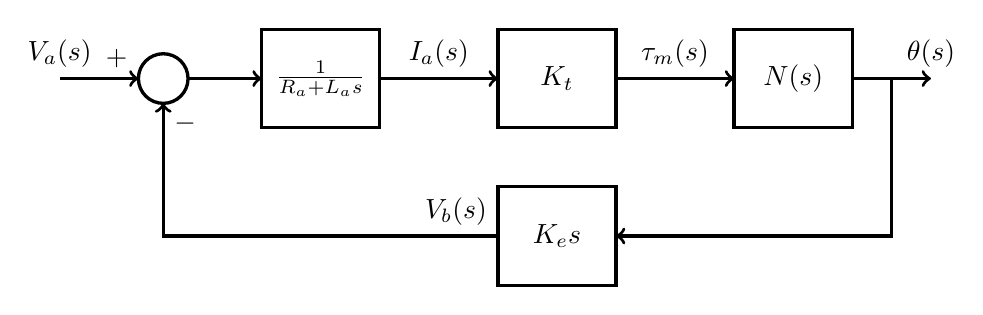
\begin{tikzpicture}[inner sep=0pt,outer sep=0pt,very thick,
sysblock/.style={draw,rectangle,inner sep=2pt,minimum width=1.5cm,minimum height=1.25cm,very thick}]

\draw (0,0) node[draw,circle] (sum) {$\rule{0pt}{18pt}$};
\draw (2,0) node[sysblock] (a) {$\frac{1}{R_{a} + L_{a}s}$};
\draw (5,0) node[sysblock] (b) {$K_{t}$};
\draw (8,0) node[sysblock] (c) {$N(s)$};
\draw (5,-2) node[sysblock] (d) {$K_{e}s$};

\draw[<-] (sum.180) node[above left=4pt] {$+$} -- ++(-1,0) node[above=4pt] {$V_{a}(s)$};
\draw[->] (sum.0) -- (a.180);
\draw[->] (a.0) -- node[pos=.5,above=4pt] {$I_{a}(s)$} (b.180);
\draw[->] (b.0) -- node[pos=.5,above=4pt] {$\tau_{m}(s)$} (c.180);
\draw[->] (c.0) -- ++(1,0) node[above=4pt] {$\theta(s)$};
\draw[->] (c.0) -- ++(.5,0) |- (d.0);
\draw[->] (d.180) node[above left=4pt] {$V_{b}(s)$} -| (sum.-90) node[below right=4pt] {$-$};

\end{tikzpicture}
\end{center}


